\section{Cutting your neck at the Guillotine}


\begin{verse}
\begin{centering}
Tired of Big Passages? \\
Fed up with crystals? \\
Enough of easy pushing? \\
Brand new oversuit with no holes? \\

Or; Just bored of life \\
   and want to try your luck? \\

Then; \\ 

Go To Push \textbf{Guillotine}! \\

Guaranteed excitement \\
Great adventure \\
Excellent for adrenalin rush \\

Join the club of survivors! \\

Now with special rewards \\
at the far end \\

Good luck and don't forget your helmet!\\
 \end{centering} \raggedleft{
Gergely Ambrus~\raisebox{-0.5em}{\protect
\includegraphics[height = 4ex]{icons/feather.png}}}
\end{verse}


\margininbox{Guillotine}{
     \begin{itemize}
    \item Gergely Ambrus
    \item Rhys Tyers
    \end{itemize}}{\explo}


It is always a long time that passes between two expeditions. A time for
living the normal life, doing the work, caving a lot, fixing or
purchasing new gear, and -- making plans for the next year.

As so much passage had been discovered within the -600 m phreatic level,
it became reasonable to hope that there might be a connection between
\passage{Sistem Migovec} and \passage{Gardeners' World} at this depth. The
\bignote{efforts for finding the connection at -400 had been failing for years},
despite the plenty of action and enormous energy that went into this
action. Meanwhile, large amounts of passages had been found at -600 with
much less effort, and sometimes they went as far as 500 m on a trip.
Therefore, it was not insane to look for the connection here.

But where could it be? Although \passage{Vrtnarija} had now several
kilometres of passages at this level, the System only intersected it.
Back in the years the primary goal was to reach the -1000 m barrier, and
it was evident looking at survey -- there were almost no horizontal
sections that had been found below 400 metres depth. There was only one
place on the survey which resembled something like \passage{Friendship
Gallery}: the area around \passage{Elephant} and \passage{Waterloo}, not far
from \passage{Hotel Tolminka}. To make things even more complicated, \bignote{these
could not be reached without changing the ropes, and we did not have the
manpower} and the gear to do so. Therefore, if one wanted to find a
connection, it had to be done from the \passage{Vrtnarija} side. Given the
dimensions of the cave, this was nothing less than finding a needle in
the haystack.

Looking at the plan of the cave, we noticed that \passage{Minotaur Rift}
was heading more or less towards \passage{Elephant}, about the same depth
level. The horizontal distance between these two points was about 250 m,
which was not so much considering the potential in the phreatic level.
Moreover, the \passage{Minotaur Rift} was formed along a huge, very well
defined fault line, which had a strong potential for continuation at
both ends. (This fault could also be found at the -800 level). It is
there that I wanted to look for the passage leading to the System!


\fullwidthbox{THE TRUE STORY OF \passage{Minestrone}}{Four lonely souls were wandering on top of Migovec searching for a cause
worthy of fighting for. Then they heard of the legend of Lost Miles and
decided to band together to create the almighty caving force of the
Fantastic Four.

The brave adventurers battled their way through \passage{Stuck in Paradise}
to reach the beautiful sandy shores of \passage{Hawaii}.

``Let's have some soup,'' said Kate.

``How about Minestrone?'' asked Gergely. All four cheer in
excitement.

``Now guys, whatever you do, don't step on this rock or the
Minestrone will go everywhere,'' Kate said in a superior air.

``Should we put one or two sachets? If we have one we can save the other
for later.''

``Two!'' said Kate.

Just as the second sachet went in and the delicious aroma of
Minestrone was wafting around \passage{Hawaii}, Kate put her clodhoppers on
the rock and toppled the almighty power source that is
Minestrone.

``Ohhhhh\ldots{}'' said Kate.

The rivers of spilt \passage{Minestrone} flowed towards the promised land
of 650 m of walking passage. And thus the passages of \passage{Minestrone}
and the beautiful \passage{Atlantis} was born.
\mininame{29/7/12 9:36am - Gergely, Kate, Rhys, Clare AKA the Fantastic Four}}



\begin{marginfigure}
\checkoddpage \ifoddpage \forcerectofloat \else \forceversofloat \fi
\centering
 \frame{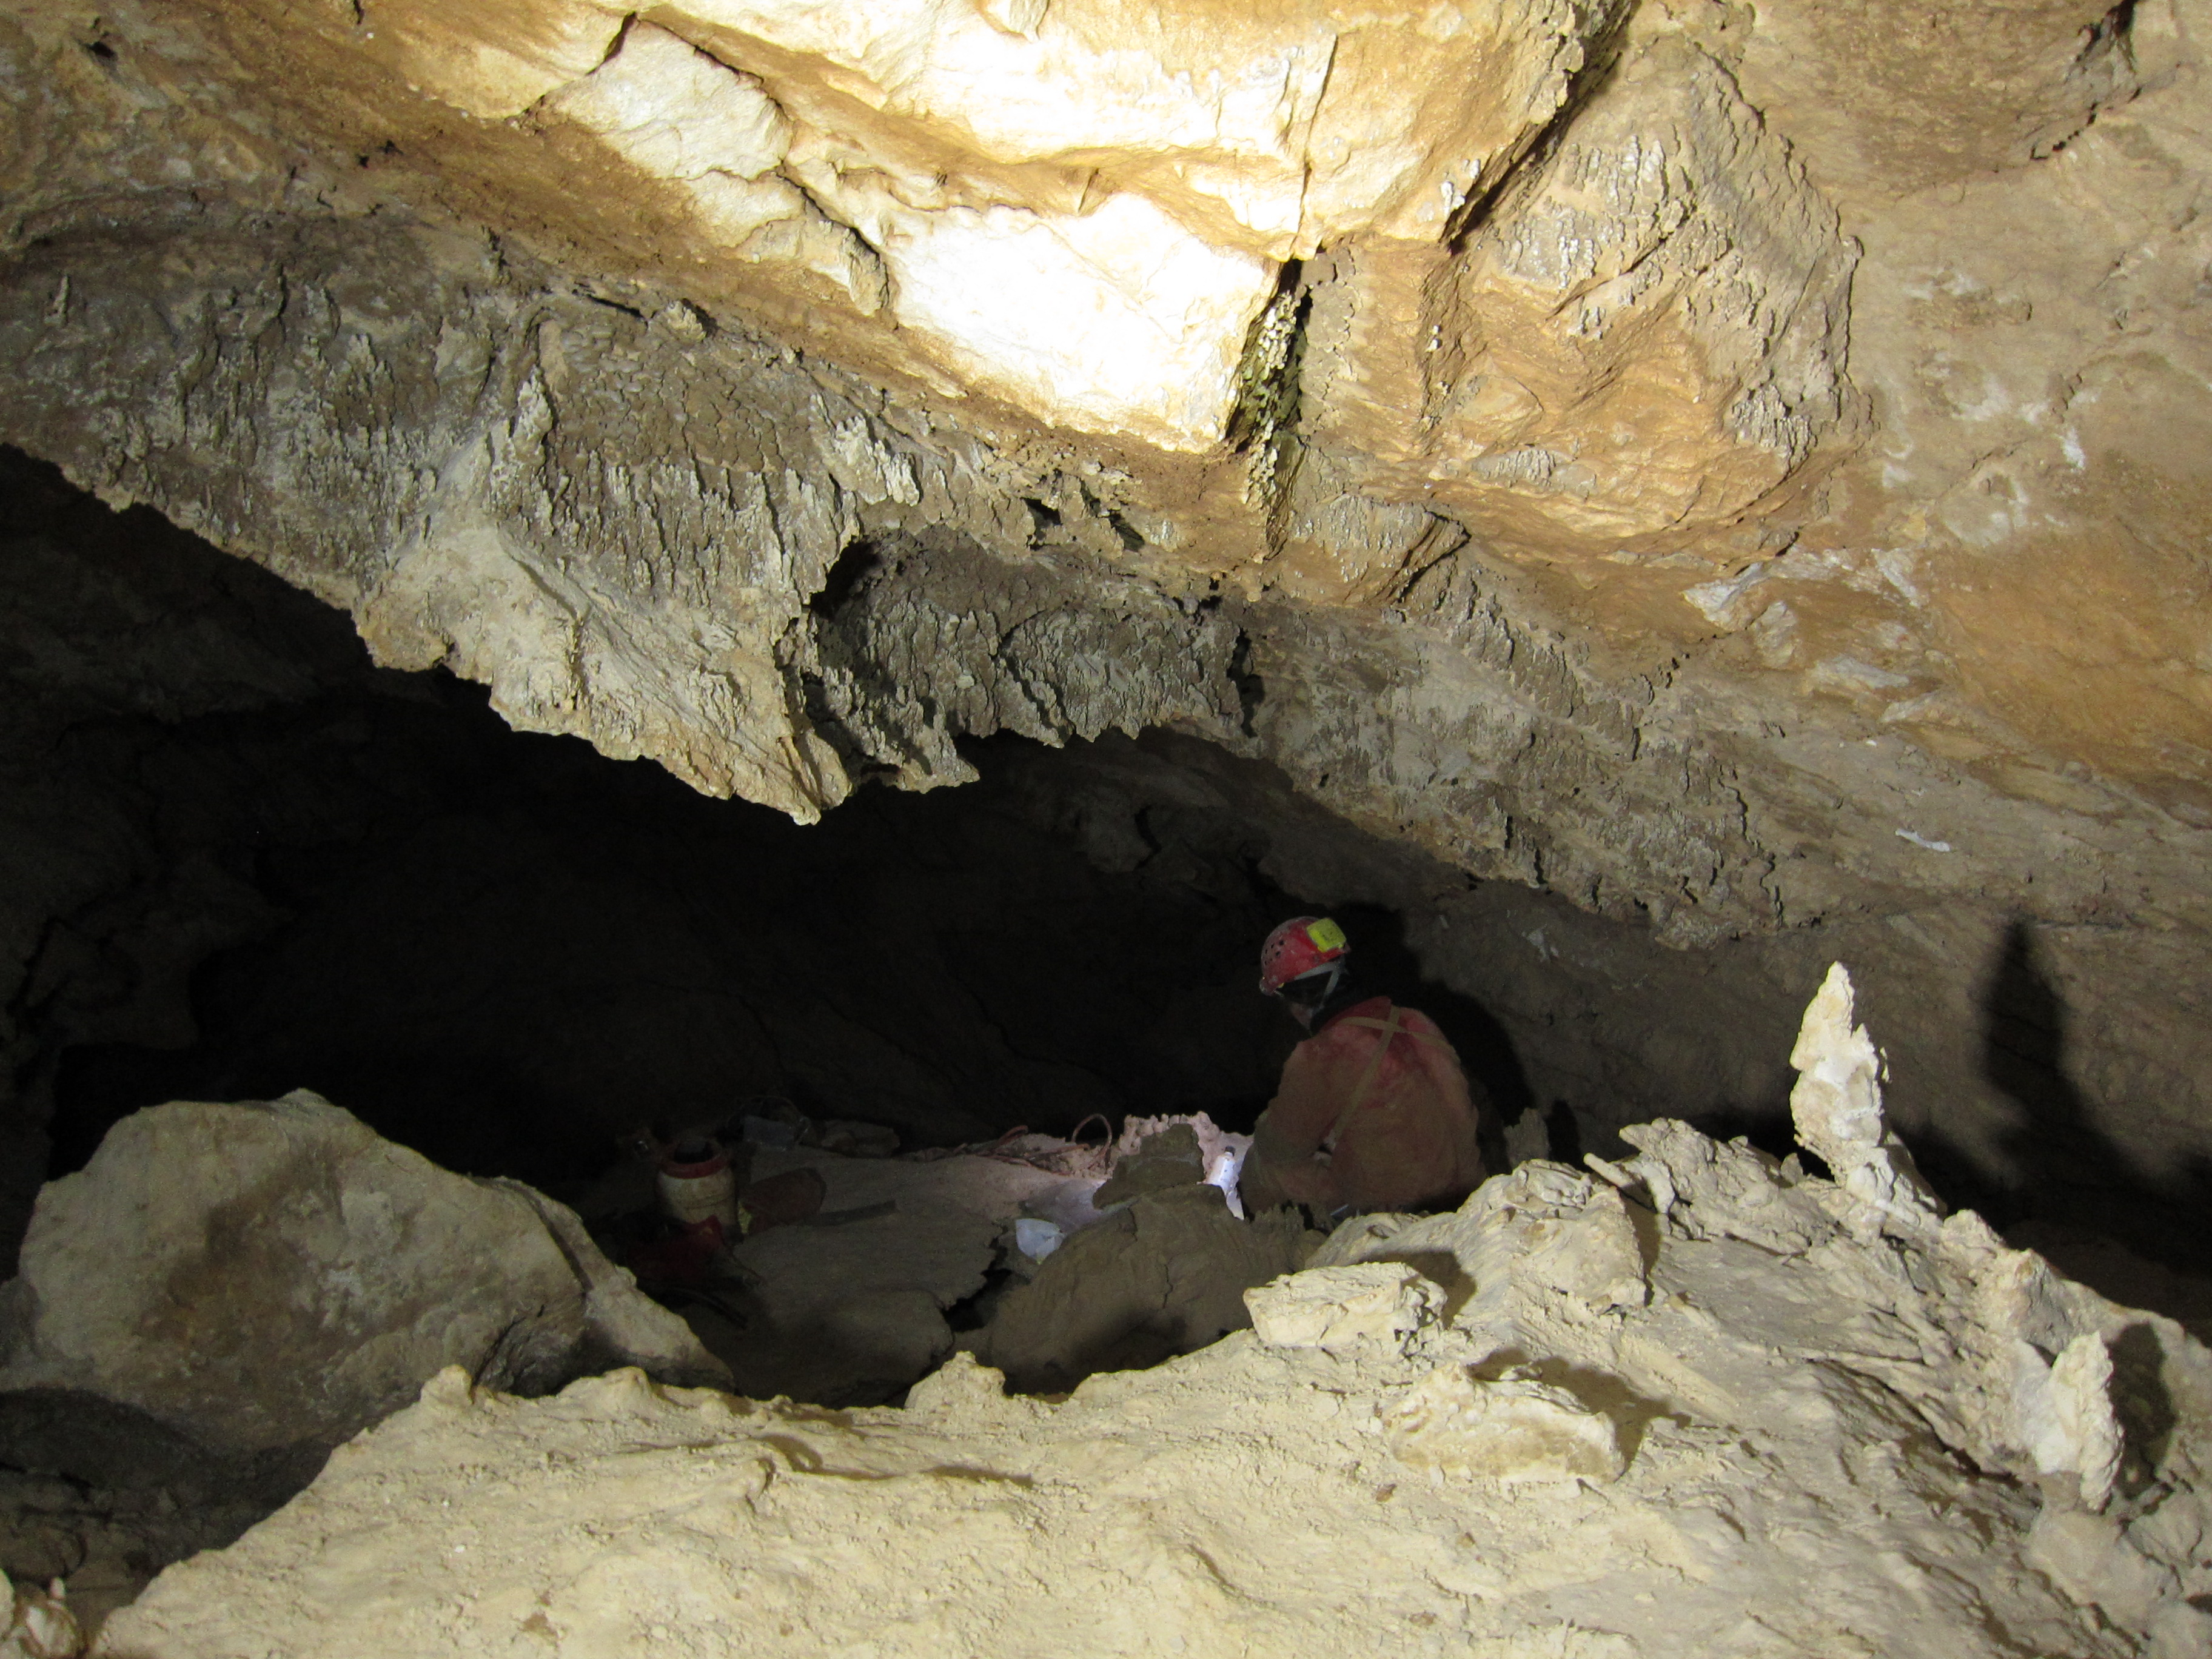
\includegraphics[width=\linewidth]{2012/guillotine/2012-08-03-0536-JanaCarga-062--orig.jpg}} 
 \caption{The passage \passage{Hawaii}. \pic{Jana Čarga}}
 \label{hawaii}
\end{marginfigure}


After the great pushing day with Kate, Clare and Rhys and finding
\passage{Atlantis}, I decided to go there with Rhys. At the end of the
\passage{Minotaur Rift}, just where the crystals appear and the passage
turns towards the right, it was possible to continue along the fault
line in a small passage. We only had to continue this line, and it was a
straightforward task to do. This has already been pushed to a boulder
choke by James Kirkpatrick. There was only one minor problem: the fault
line itself! For obvious reasons, the rock there was extremely loose and
broken. So, on one hand, we had to move a lot of rocks in order to make
progress, but on the other hand, we were never quite sure whether the
ceiling was going to collapse on us or not.

There was one point along the passage, where we needed to squeeze down
on the left hand side. We managed to move quite a number of rocks, but
one large one remained there, and there was nothing for it but to
squeeze underneath. When I finally attempted to pass under this rock
blade, of course it moved\ldots{} but luckily, by not so much. Since
there was no space for putting the rock anywhere else, we tried to stack
smaller rocks underneath in order to keep it up. Still, \bignote{when you
climbed, your head was directly under it}\ldots{} good luck! So, the name
of the passage became \passage{Guillotine}!

Eventually, after long hours of battling against the rocks, we managed
to emerge in an open space: the fault line opened up again! We found
ourselves at the top of a $\approx$ 30 m high rift, with an
active streamway, with beautiful white walls! In the squeeze, we found
haematite pebbles and in some places along the fault line, the rock
looks like marble, which would be very nice were it not for the fact
that it constantly rains down on your head. Crawling out from
\passage{Guillotine} was even harder than going in, since the whole passage
was sloping downwards. Moreover, as we crawled, the oversuits became
packed with sharp little rocks, while other rocks constantly fell on our
heads. A truly fascinating place! Still, the continuation was at the
bottom of a large, open and going rift -- quite the lead\ldots{}



\margininbox{Razor}{
     \begin{itemize}
    \item Gergely Ambrus
    \item Rhys Tyers
    \end{itemize}}{\explo}


Later, we returned with Jana to rig the rift at the end, and to survey
the passage. The end of the rift needed some bolt climbing, but we could
hear that it continued on with large volumes. Moreover, to our surprise,
the passage went more than 100 metres in the direction of the System!
Thus, the distance to the connection became less than 120 metres. We
then planned to go back there to climb up the following year. Thanks
God, the events that followed later made this heroic attempt unnecessary
(since \passage{Sanje za Duso}\sidenote{\passage{Dreams for the Soul}}
crosses the continuation of the rift). It is thus likely that nobody
will ever enjoy the special treatment of \passage{Guillotine} again. Who
knows, maybe since then, the large boulder has already fallen down,
sealing the passage for eternity\ldots{}

\name{Gergely Ambrus}



    \begin{pagefigure}
\checkoddpage \ifoddpage \forcerectofloat \else \forceversofloat \fi
    \centering
        \frame{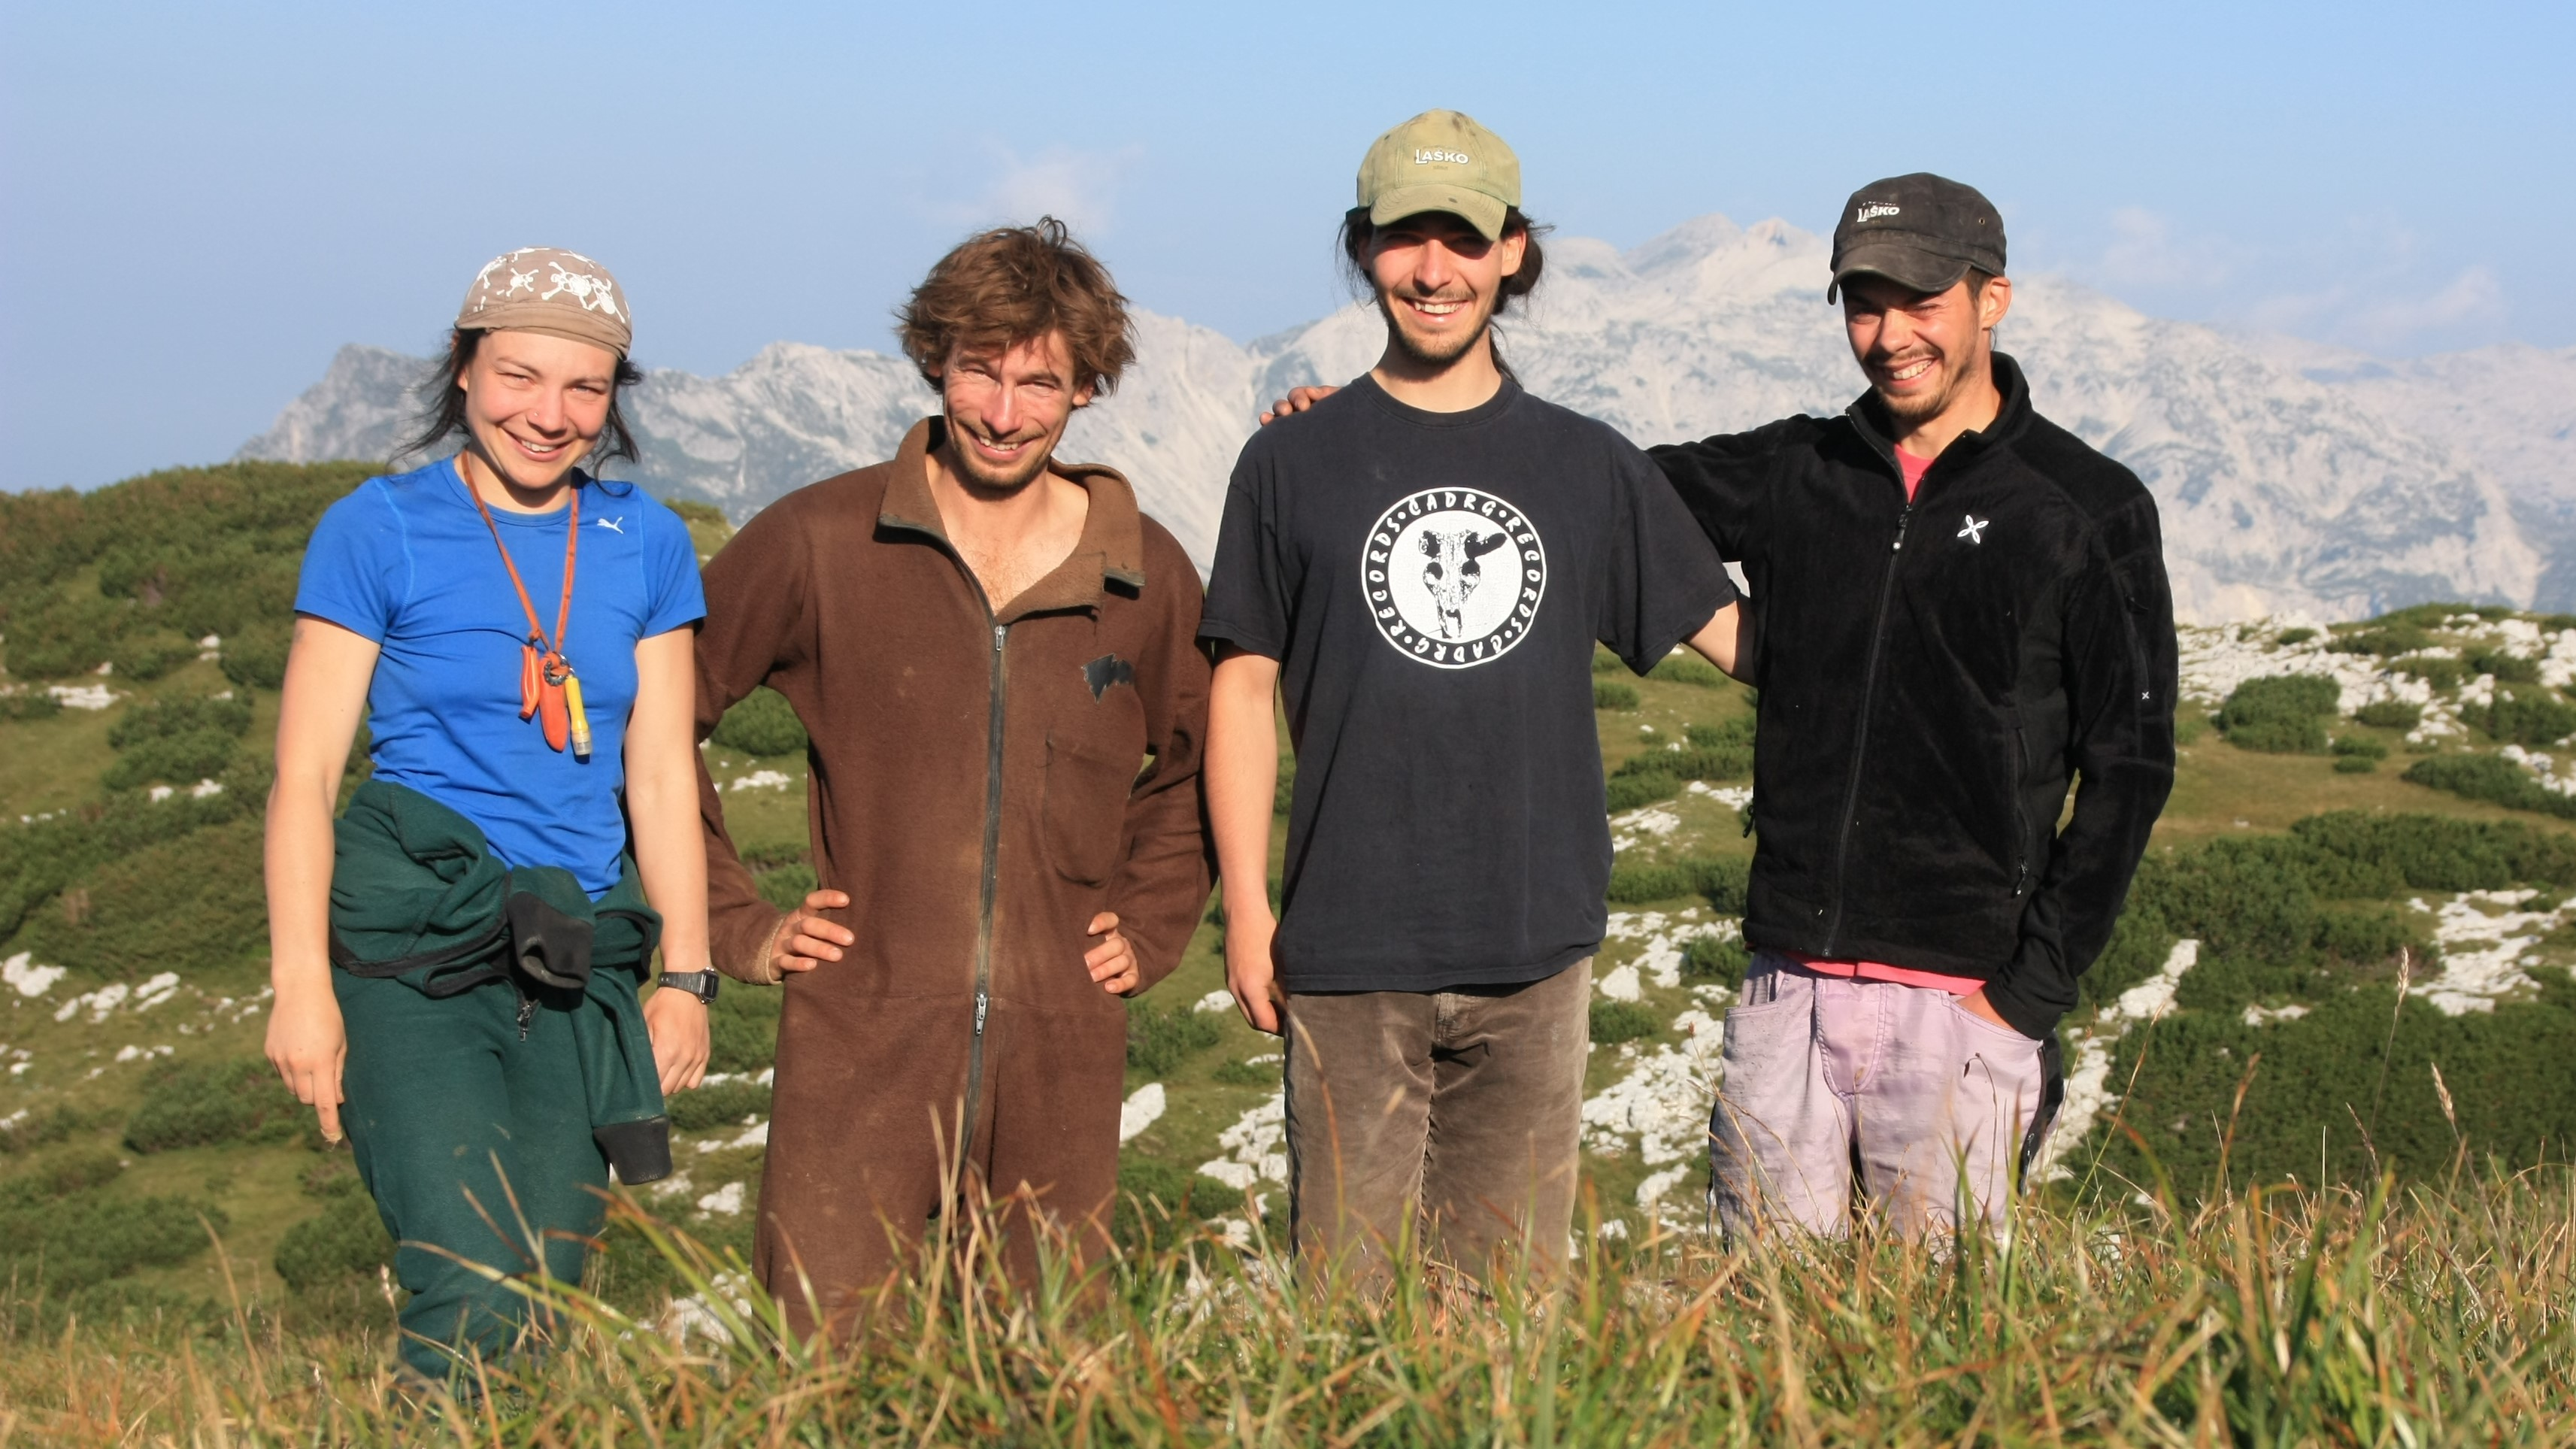
\includegraphics[width=\linewidth]{2012/guillotine/2012-08-03-2305-GergelyAmbrus-IMG_2196--orig.jpg}} 
        \caption{Team Eastern European: Jana, Gergely, Izi and Maver. \pic{Gergely Ambrus}} \label{eastern european quartet}
    \end{pagefigure}
